\chapter{Ein traditioneller Compiler}

Ein Compiler ist traditionell mit folgendem Schema beschreiben.

\begin{figure}[h!]
    \centering
    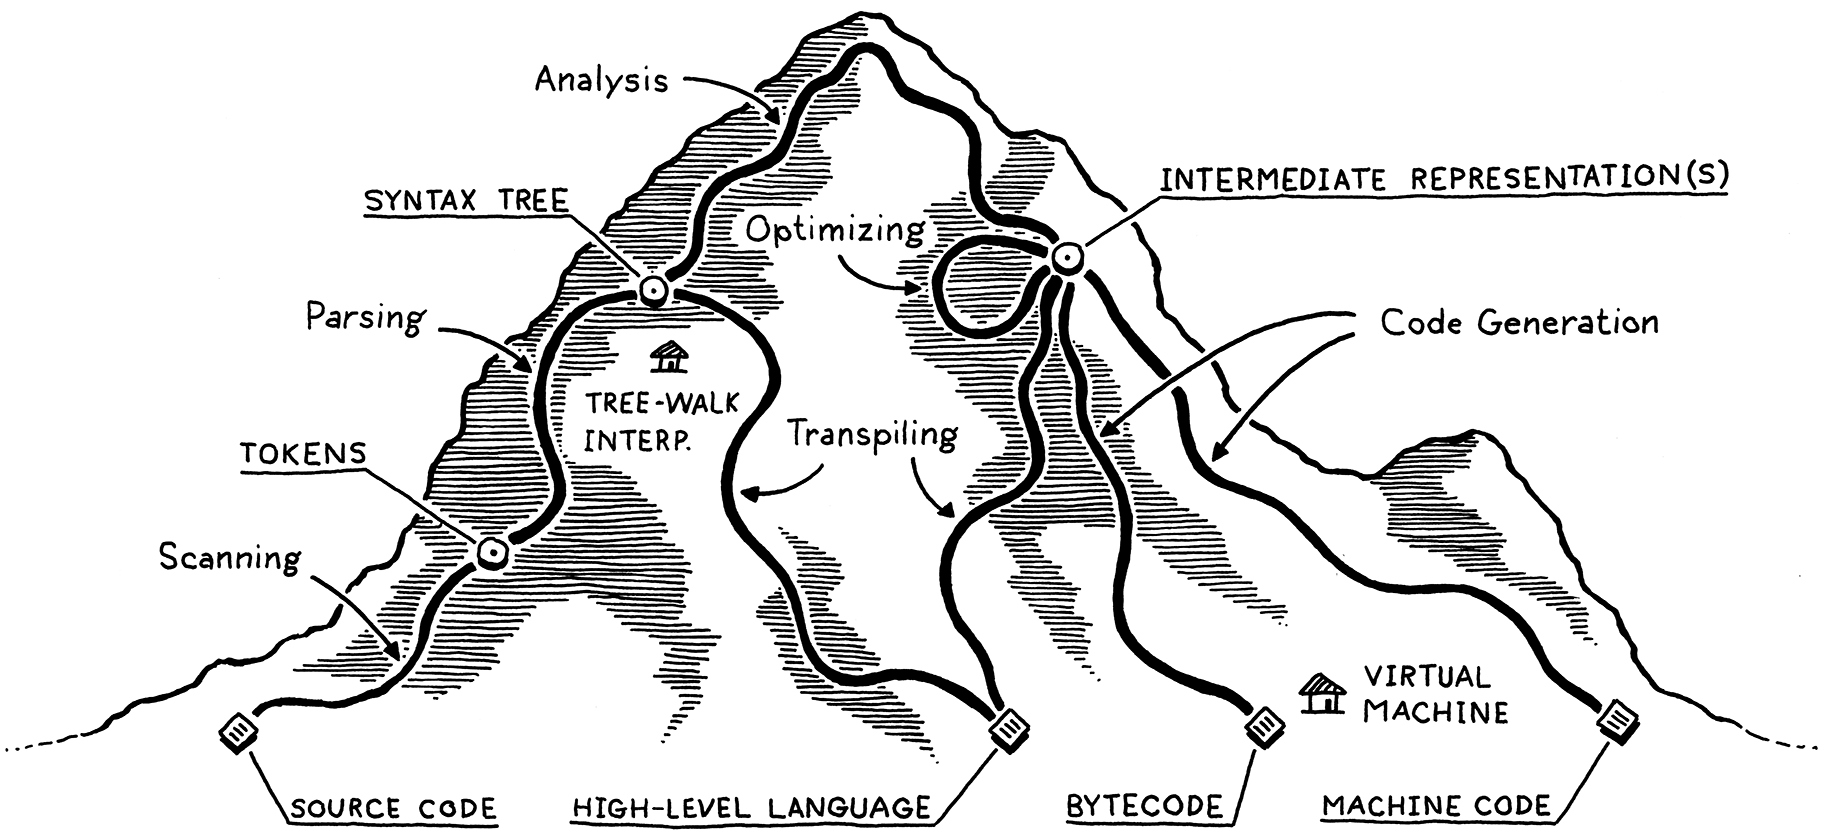
\includegraphics[scale=0.2]{resources/images/mountain.png}
    \caption[Schritte, die ein Compiler durchläuft (https://github.com/munificent/craftinginterpreters, besucht am 5.8.2024)]{Schritte, die ein Compiler durchläuft}
    \label{fig:mountain}
\end{figure}

In dieser Arbeit werde ich mich nur auf die im unteren Schema \ref{fig:mountain-edited} dargestellten Schritte fokussieren.

\begin{figure}[h!]
    \centering
    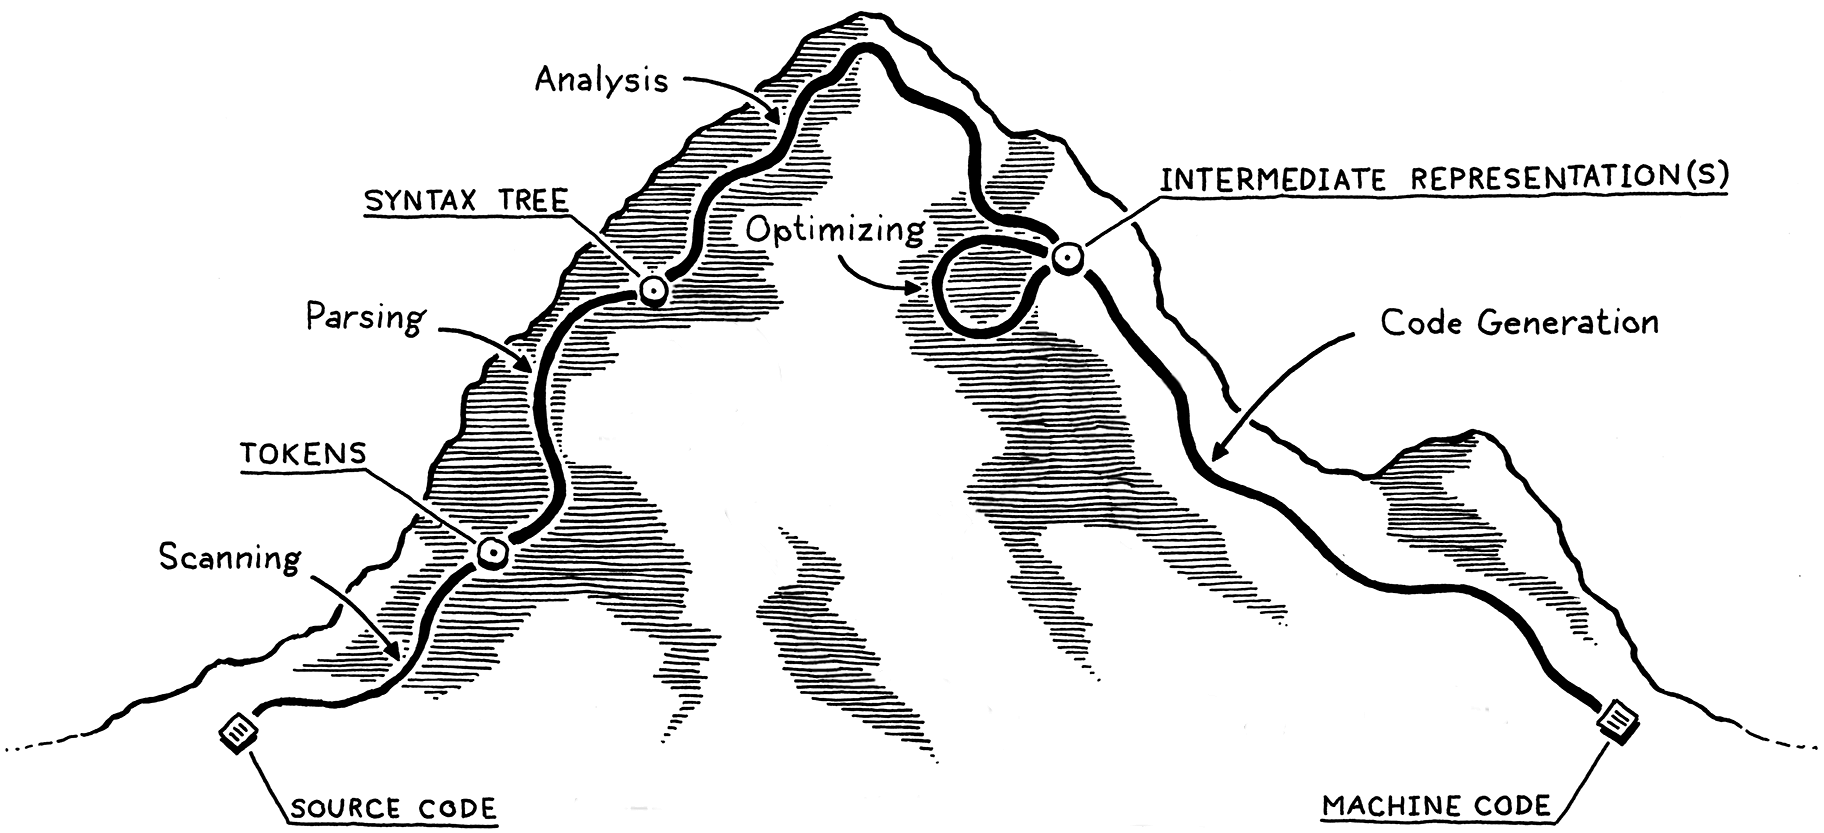
\includegraphics[scale=0.2]{resources/images/mountain-edited.png}
    \caption[Schritte, die in dieser Arbeit behandelt werden (Basierend auf Bild \ref{fig:mountain})]{Schritte, die in dieser Arbeit behandelt werden}
    \label{fig:mountain-edited}
\end{figure}

\section{Lexical Analysis}
Meist werden Programme so geschrieben, dass wir Menschen sie lesen und verstehen können. Dafür verwendet man Buchstaben, Zahlen, Zeichen, wie + oder *, und Whitespaces, wie Leerzeichen oder Absätze.
Diese sind jedoch für den Computer noch nicht sofort verständlich. Der erste Schritt beim Kompilieren ist daher die \textit{Lexical Analysis}. Dies wird von einem Teil des Compilers, dem \textit{Lexer}, durchgeführt.
Die Aufgabe dieses Lexers ist es den Inputfile zu analysieren und die gefundenen Zeichen in sogenannte \textit{Tokens} zu verwandeln. Diese Tokens sind Datenstrukturen, die der Compiler kennt und mit denen er weiterarbeiten kann.

Als Beispiel:

\begin{lstlisting}[language=C, label=eg:preLex, caption=C code vor Lexical Analysis]
int foo()
{
    if (bar == 0)
    {
        return 0;
    }

    return 1;
}
\end{lstlisting}

\begin{lstlisting}[label=eg:postLex, caption=Tokens nach Lexical Analysis]
Keyword         (keyword="int")
Identifier      (id="foo")
LParenthesis
RParenthesis
Keyword         (keyword="if")
LParenthesis
Identifier      (id="bar")
Operator        (operator=ComparisonEqual)
LiteralInt      (value=0)
[...]
\end{lstlisting}

Der Lexer legt hierbei fest welche Zeichen die Input-Programmiersprache enthalten darf und welche Bedeutung ihnen zugesprochen wird. So ist zum Beispiel im Lexer festgelegt, dass ein + Zeichen als Addition interpretiert wird.
Genauso wie im Listing \ref{eg:postLex} 'if' als KeywordToken gesehen wird, lässt sich im Lexer auch bestimmen, dass ein Wort wie 'print' als Keyword angesehen werden soll.

\section{Syntax Analysis}
Nun versteht der Compiler was mit den Zeichen im Inputfile gemeint ist, jedoch fehlt noch etwas bis tatsächlich in eine andere Programmiersprache übersetzt werden kann. Und das ist Verständnis für Syntax.
Die meisten High-Level Programmiersprachen weisen Syntaxregeln auf. Diese beinhalten, wie Funktionen und Variablen definiert werden oder mit welchen Punktvorstrich-Regeln Expressions evaluiert werden.
In diesem Schritt für der sogenannte \textit{Parser} die \textit{Syntax Analysis} durch.
Hierbei werden die bei der Lexical Analysis gefundenen Tokens ineinander verschachtelt und in einen sogenannten \textit{Abstract Syntax Tree (AST)} überführt.

\begin{figure}[H]
    \centering
    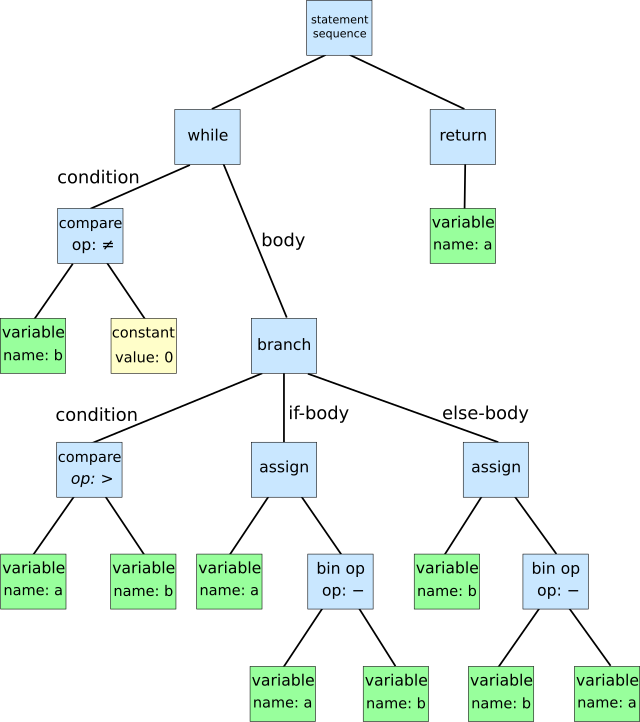
\includegraphics[scale=0.3]{resources/images/syntaxtree.svg.png}
    \caption[Abstract Syntax Tree (https://en.wikipedia.org/wiki/Abstract\_syntax\_tree, besucht am 5.8.2024)]{Abstract Syntax Tree zum Euklidischen Algorithmus}
    \label{fig:syntax-tree}
\end{figure}

Ein AST enthält somit nicht nur Informationen über die Tokens, sondern über die gesamten Strukturen und Abhängigkeiten, die sich aus den Tokens ergeben. Variabel- und Funktionsdefinitionen oder komplexe Statements wie 'if' oder 'for'
sind im AST als \textit{Nodes} enthalten. Wenn man die Nodes des AST von unten nach oben durchquert, erhält man die Reihenfolge der einzelnen Tokens ohne Abhängigkeitskonflikte.
Eine Subtraktion kann zum Beispiel erst ausgeführt werden, wenn sowohl die linke als auch die rechte Zahl bekannt ist.
Daher befindet sich, wie in Abbildung \ref{fig:syntax-tree} ersichtlich, die Subtraktion über den beiden benötigten Werten im AST.

\section{Semantic Analysis}
Semantik ist die Wissenschaft der Bedeutung von Worten einer Menschensprache. Bei einem Compiler geht es bei der \textit{Semantic Analysis} weniger um Bedeutung und mehr um die Konsistenz von Datentypen.
In diesem Schritt der Kompilierung beschäftigt sich der Compiler mit der Korrektheit von Expressions.
Wird eine Variable nicht konform ihres Datentyps verwendet, zum Beispiel die Division zweier Strings, wird dies während der Semantic Analysis entdeckt und gemeldet.
Auch werden unbekannte Variablen und Funktionen in diesem Schritt abgefangen.
Weiter wird der Datentyp einer Node an diese angebunden. Gegebenenfalls kann auch ein impliziter Cast, also ein impliziter Wechsel des Datentyps hinzugefügt werden.
So geben zum Beispiel manche Programmiersprachen bei der Division zweier Integers eine Float zurück.

\section{Code Generation}
Code Generation ist der finale und oft auch komplexeste Schritt, der ein Compiler ausführen muss. Nun da unser Input-Code nicht mehr nur als Textfile, sondern als Intermediate Representation vorliegt,
kann endlich Output-Code generiert werden. Jedoch lässt sich über diesen Schritt fast am wenigsten sagen, da er je nach Output-Sprache sehr unterschiedlich aussehen kann. 
[Code generation types]

\section{Optimization}
Code Generation ist zwar der letzte Schritt beim Kompilieren, trotzdem wurde eine wichtige Aufgabe des Compilers noch nicht betrachtet. \textit{Optimization} geschieht zwischen jedem der genannten Schritte und dies häufig mehrmals.
Dabei geht es darum den Output-Code so effizient wie möglich zu machen. Effizient kann hierbei viel Verschiedenes bedeuten. Der Output-Code muss so schnell wie möglich ausgeführt werden,
Memory sparsam verwenden und am besten auch noch eine möglichst kleine Datei sein. Optimization reicht vom Entfernen der Kommentare und Umstellen von mathematischen Operationen bis zu entfernen von ungebrauchten Variablen und Deadstores.
Es muss von CPU Registern profitiert, mit Heap-Memory umgegangen und von inline Funktionen Gebrauch gemacht werden. Compiler Optimization ist somit ein sehr vielseitiges und komplexes Problem,
dass hierbei nicht weiter thematisiert werden sollte.